\subsection{Прогноз и характеристика рынка Интернета вещей в 2019}
\label{sec:analysis:data_art}

В ноябре 2018 года компания DataArt, специализирующаяся на аутсорсинге разработки ПО и таких областях, как интернет-приложения, корпоративные базы данных и инструменты промышленной автоматизации, представила прогноз по развитию рынка интернета вещей в 2019 году.

По словам экспертов, когда-то интернет вещей был нишевой технологией для стартапов, а теперь на ее основе строят бизнес корпорации с оборотом в миллионы долларов. IoT уже изменил жизнь, а 2019 год должен стать периодом значительных перемен в этой области. IoT-специалисты DataArt назвали основные тенденции, которые будут преобладать на рынке интернета вещей в 2019 году.

Устройства станут еще мощнее, обеспечивая локальную обработку данных и возможности искусственного интеллекта. Это уменьшит объемы передачи данных и зависимость от облачных вычислений, а также предоставит больше гибкости компаниям. Граничные вычисления окажут существенное влияние на те отрасли, где необходимо немедленное реагирование, основанное на сложном анализе данных в режиме реального времени (например, производство и общественная безопасность), и там, где облачные коммуникации могут быть ограничены (доставка, логистика и т. п.) \cite{iot_data_2019}.

Ключевым шагом на пути к трансформации отрасли станет гонка компаний, которые будут соперничать в разработке наиболее эффективных и безопасных IoT-решений. Специалисты по IoT-рынку сконцентрируются на решении ключевых проблем безопасности и устранении уязвимостей, связанных с Интернетом вещей, которые прежде препятствовали широкому распространению технологии.

По прогнозам DataArt, в 2019 году будет заметна обостренная конкуренция между технологическими гигантами, вроде Amazon Web Services (AWS), Microsoft и Google, поскольку большие IoT-платформы стали обычным явлением. Такие корпорации смогут захватить большую часть рынка и продолжать расширять зону влияния за счет примыкающих к ним организаций. На фоне борьбы за рыночную долю среди крупных производителей IoT-платформы небольшие компании вынуждены будут для выживания сосредоточиться на нишевых областях (например, перемещение данных, решение специфических проблем в выбранных отраслях, работа с определенными типами устройств и т. д.) \cite{iot_data_2019}.

Аналитики говорят, что в различных отраслях «умные» устройства бесспорно станут еще популярнее. Ожидается растущее использование такой электроники в автомобильном, промышленном, медицинском, производственном и других секторах (Рисунок \ref{fig:analysis:forecast:deviceDiagram}).

~
\begin{figure}[H]
\centering
	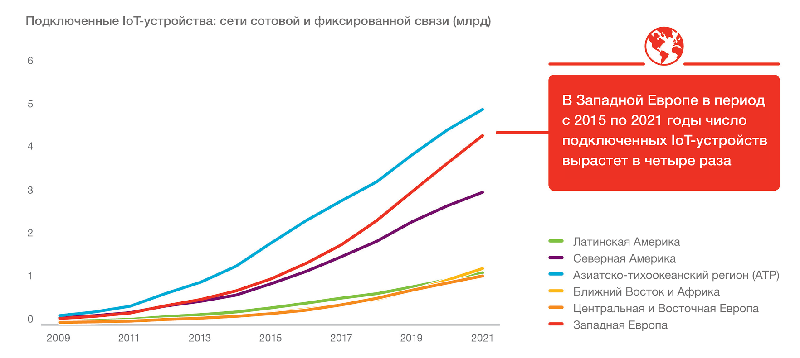
\includegraphics[scale=0.8]{figures/forrester.png}
	\caption{Список подключенных IoT устройств в мире}
	\label{fig:analysis:forecast:deviceDiagram}
\end{figure}

Данные становятся жизненно важной основой автомобильной промышленности. Участники рынка будут и дальше активно внедрять IoT-технологии, чтобы обеспечить машинам незаметный сбор и мониторинг данных, а также их взаимодействие с сервисами «умного» города и другими транспортными средствами.

5G-сети, которые считаются одной из самых ожидаемых технологических тенденций, откроют новую эру для Интернета вещей, способствуя усилению взаимосвязи элементов современного мира. Это приведет к дальнейшему развитию IoT-инноваций, что даст возможность собирать данные, анализировать их и управлять ими практически в режиме реального времени \cite{iot_data_2019}.

Число вендоров, стремящихся занять часть рынка IIoT, продолжает расти, но некоторые лидеры вышли из поля, говорится в другом исследовании, опубликованном на этой неделе. Согласно отчету Forrester Research о программных платформах IIoT, C3 IoT, Microsoft, PTC, SAP и IBM являются лидерами отрасли, при этом самое сильное предложение делает C3 IoT, а IBM намного опережает других поставщиков по стратегии. Amazon Web Services считается только «претендентом» на пространство IIoT, оставшись позади сильнейших игроков, таких как GE, Oracle и Siemens. Forrester поставила Cisco на последнее, 15-е место среди компаний по ассортименту и стратегии. Вендоры оценивались по 24 критериям, включая аналитические возможности, использование технологии цифровых двойников и производственную интеграцию \cite{iot_data_2019}.

Эксперты говорят, что в предыдущие годы эта технология быстро развивалась благодаря широкому распространению сенсоров, а также инфраструктур облачных и периферийных вычислений. В результате интернет вещей стал менять не только бизнес компаний, но и жизнь обычных людей. Ниже представлены пять тенденций, которые, по мнению исследователей, будут преобладать в сфере IoT и оказывать влияние на организации и предприятия.

В Forrester считают, что концепция централизованного «умного» дома, в котором устройства тесно взаимодействуют между собой, стала мечтой скорее компаний, чем потребителей. Интерес к рынку оборудования для «умных» домов снижается со стороны домашних пользователей, которые предпочитают покупать только одно многофункциональное устройство, управляемое при помощи приложения. Такая тенденция, скорее всего, сохранится в 2019 году. Но компании могут попытаться объединять услуги в пакеты и привлекать клиентов скидками, но люди пока не готовы к такого рода интегрированным коммуникациями, говорится в докладе, выпущенном в ноябре 2018 года \cite{iot_data_2019}.

По словам аналитиков, разговоры об интернете вещей как о непонятном модном термине уйдут на второй план, а на первом — появятся проекты реального применения технологии.

Аналитики считают, что в 2019 году разработчики IoT-платформ будут сужать сферу своей деятельности, сосредотачиваясь на определенных вариантах использования. Например, бизнесменам не нужна одна единственная платформа промышленного интернета вещей для управления каждым процессом в своей компании. Вместо этого они ищут решения, специализирующиеся на конкретных задачах. В связи с этим в 2019 году стоит ожидать еще больше партнерских соглашений с IoT-вендорами.

Еще одним трендом 2019 года эксперты называют кибератаки на системы «умных» городов. Многие города не в состоянии обеспечить безопасность подключенных устройств, датчиков и инфраструктуры связи, а также конфиденциальность граждан в системах умного города. Специалисты прогнозируют увеличение числа целенаправленных атак с помощью программ-вымогателей против уязвимых компонентов развертывания интеллектуальных городов, что приведет к сбоям в обслуживании граждан и заставит города вкладываться в кибербезопасность, чтобы свести к минимуму риск дальнейших атак \cite{iot_data_2019}.

В Forrester видят зарождение рынка услуг по управлению и эксплуатации фрагментированных IoT-объектов.